\chapter{Contextualisation}
\markboth{CHAPITRE 1. Contextualisation}{

\section{Présentation des données}

Notre jeu de données contient les informations relatives aux TER en circulation dans différentes régions de France. Ces informations sont mensuelles, et nous disposons d'un nombre d'observations différent selon la région concernée (\textit{cf Figure 1.1}).\\

\begin{figure}[H]
  \centering
  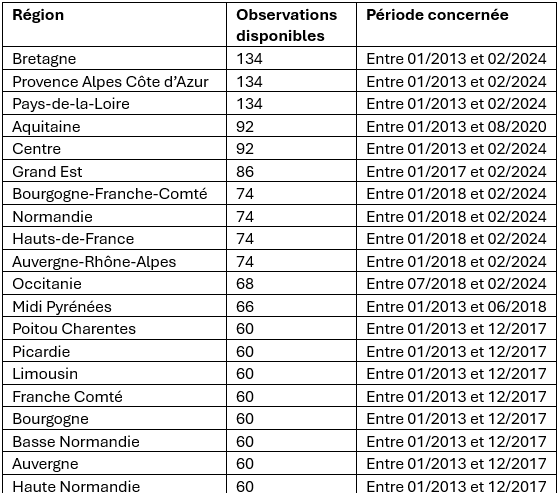
\includegraphics[width=0.8\textwidth]{Tableau_1_1.png}
\end{figure}

\begin{figure}[H]
  \centering
  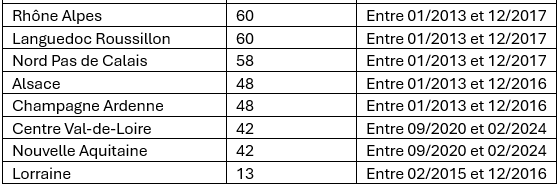
\includegraphics[width=0.8\textwidth]{Tableau_1_2.png}
  \caption{Nombre d'observations en fonction de la région}
\end{figure}

Dans notre rapport, nous considérons seulement les régions pour lesquelles nous avons plus de 70 observations (les autres régions sont traitées dans le code joint au rapport). Pour chacune de  ces régions, nous nous intéressons en particulier aux variables \textbf{'nombre de trains programmés'} et\textbf{ 'nombre de trains annulés'}. Ces variables constituent des séries temporelles auxquelles nous appliquerons notre modèle de rupture.

\section{Modèle de rupture}

Nous souhaitons appliquer notre modèle de rupture aux séries temporelles correspondant au nombre de trains programmés et au nombre de trains annulés pour les régions sélectionnées.\\

Nous utilisons un \textbf{modèle de rupture pour la loi normale asymétrique}. La densité de la loi normale asymétrique est de la forme:
\[
f(x,\mu,\sigma,\theta) = \frac{2\phi\left(\frac{x-\mu}{\sigma}\right)\Phi\left(\theta\left(\frac{x-\mu}{\sigma}\right)\right)}{\sigma}
\]
où $\phi(x) = \frac{1}{\sqrt{2\pi}}e^{-\frac{x^2}{2}}$ et $\Phi(x) = \int_{-\infty}^{x} \phi(t)dt$.\\

Nous considérons le modèle suivant :
\[
\begin{cases}
X_t \sim \mathcal{SN}(\mu_1,\sigma_1,\theta) & \text{si } t \leq k \\
X_t \sim \mathcal{SN}(\mu_2,\sigma_2,\theta) & \text{si } t > k
\end{cases}
\]
où $\mu_1$, $\sigma_1$, $k$, $\mu_2$, $\sigma_2$, $\theta$ sont inconnus que l'on souhaite estimer.\\

Concrètement, nous suivons la démarche suivante:

\begin{itemize}
  \item Soit k, un moment de rupture supposé. Nous évaluons les paramètres des lois normales asymétriques des variables aléatoire $X_1, ..., X_k$ et $X_{k+1}, ..., X_n$ en nous basant sur les échantillons dont nous disposons.
  \item Nous souhaitons déterminer $\hat{k}$, le moment de rupture le plus probable. Pour cela, nous évaluons les paramètres des lois normales asymétrique pour chaque k candidat (c'est à dire appartenant à $\llbracket 10, n-10 \rrbracket$ ). Nous sélectionnons alors k tel que les lois obtenues en considérant ce moment de rupture soient le plus plausible.
  \item Ayant déterminé $\hat{k}$, nous testons la similarité en loi des échantillons ($x_1, ..., x_{\hat{k}}$) et ($x_{\hat{k}+1}, ..., x_n$).
\end{itemize}

La mise en œuvre de chaque étape est détaillée dans le chapitre suivant.


}


